\documentclass[aspectratio=169]{beamer}
\usepackage{lmodern}
\usetheme{Madrid}
%\usecolortheme{giantoak}
\newcommand*\oldmacro{}
\let\oldmacro\insertshorttitle
\renewcommand*\insertshorttitle{\oldmacro\hfill\insertframenumber\,/\,\inserttotalframenumber}
\usepackage[framemethod=tikz]{mdframed}

\usepackage{beamerthemesplit}
\usepackage{textpos}
\usepackage{pgf}
%\logo{\pgfputat{\pgfxy(0,-.4)}{\pgfbox[right,base]{\includegraphics[height=1.0cm]{logo.jpg}}}}
%\newcommand{\nologo}{\setbeamertemplate{logo}{}}
\usepackage{booktabs}
\usepackage{graphicx}
\theoremstyle{principle}
\newtheorem*{principle}{Design Principle}


\titlegraphic{\includegraphics[width=1.0\paperwidth]{cool-wind-800px.jpg}}

\title{Amendments}
%\author[Jeremy Kedziora]{Wind Data Science Team\\
%\small{Uptake}}
\date{}

\begin{document}

%{
%%\nologo
%\begin{frame}
%    \maketitle
%\end{frame}
%}
%pages 1-7, 8-9, 14-15.


{
  \usebackgroundtemplate{
\includegraphics[width=1.0\paperwidth]{gov.jpg}}
  \begin{frame}[plain]
  
\begin{mdframed}[tikzsetting={draw=black,fill=white,fill opacity=0.7,
               line width=0pt},backgroundcolor=none,leftmargin=20,
               rightmargin=20,innertopmargin=4pt]
\Huge Things Governments Do
\end{mdframed}

  \end{frame}
}

%@@@@@@@@@@@@@@@@@@@@@@@@@@@@@@@@@@@@@@@@@@@@@@@@@
\begin{frame}
\frametitle{Birkland$+$ Model of Policy}
\begin{itemize}
\item Policy Domain: what substantive problems are under consideration (e.g. water pollution, defense, etc.)???
\begin{itemize}
\item This specifies:
\begin{itemize}
\item The actors involved, official actors who can make decisions $+$ stakeholders; 
\item Their organization, e.g. iron triangle, policy community;
\item The systemic agenda; 
\item The distribution of benefits and costs;
\end{itemize} 
\end{itemize}
\bigskip
\item \color{black}Input-output Model;
\begin{itemize}
\item Actors: legislature, executive, bureaucrats, justices and the available levers;
\item Inputs: agenda setting (application of power/social construction, focusing events, indicator change driven esp by unofficial actors) specifies the institutional and decision agendas;
\item Black box decision making (structured by median voter thm, Arrow's thm) works on the decision agenda;
\begin{itemize}
\item timing resembles incrementalism if driven by indicator change;
\item timing resembles punctuated equilibrium if driven by focusing events;
 \end{itemize}
\item Outputs (e.g. statute laws, rules, court decisions);
\end{itemize}
\bigskip
\item Feedback and iteration.
\end{itemize}
\end{frame}

%@@@@@@@@@@@@@@@@@@@@@@@@@@@@@@@@@@@@@@@@@@@@@@@@@
\begin{frame}
\frametitle{Birkland$+$ Model of Policy}
\begin{itemize}
\item Policy Domain: what substantive problems are under consideration (e.g. water pollution, defense, etc.)???
\begin{itemize}
\item This specifies:
\begin{itemize}
\item The actors involved, official actors who can make decisions $+$ stakeholders; 
\item Their organization, e.g. iron triangle, policy community;
\item The systemic agenda; 
\item The distribution of benefits and costs;
\end{itemize} 
\end{itemize}
\bigskip
\item \color{black}Input-output Model;
\begin{itemize}
\item Actors: legislature, executive, bureaucrats, justices and \textbf{the available levers};
\item Inputs: agenda setting (application of power/social construction, focusing events, indicator change driven esp by unofficial actors) specifies the institutional and decision agendas;
\item Black box decision making (structured by median voter thm, Arrow's thm) works on the decision agenda;
\begin{itemize}
\item timing resembles incrementalism if driven by indicator change;
\item timing resembles punctuated equilibrium if driven by focusing events;
 \end{itemize}
\item Outputs (e.g. statute laws, rules, court decisions);
\end{itemize}
\bigskip
\item Feedback and iteration.
\end{itemize}
\end{frame}

%@@@@@@@@@@@@@@@@@@@@@@@@@@@@@@@@@@@@@@@@@@@@@@@@@
\begin{frame}
\frametitle{Taxes}
\begin{itemize}
\item Raise revenue;
\bigskip
\bigskip
\bigskip
\item Fix market externalities;
\bigskip
\bigskip
\bigskip
\item Can create deadweight loss.
\end{itemize}

\end{frame}

%@@@@@@@@@@@@@@@@@@@@@@@@@@@@@@@@@@@@@@@@@@@@@@@@@
\begin{frame}
\frametitle{Regulation}
\begin{itemize}
\item Natural monopoly regulation to avoid price distortions, e.g. telephone company prices;
\bigskip
\bigskip
\bigskip
\item Social regulation to correct for market inefficiency, e.g. bank solvency;
\bigskip
\bigskip
\bigskip
\item Oligopolistic regulation, e.g. entry, exit, price, and service levels in a competitive industry -- require coordinating activity of many firms.
\end{itemize}

\end{frame}

%@@@@@@@@@@@@@@@@@@@@@@@@@@@@@@@@@@@@@@@@@@@@@@@@@
\begin{frame}
\frametitle{Subsidies and Grants}
\begin{itemize}
\item Incentive effects, you want to generate activity that markets/volunteerism cannot provide in adequate quantity;
\bigskip
\bigskip
\bigskip
\item Wealth effects, e.g. redistribution;
\bigskip
\bigskip
\bigskip
\item There may be tradeoffs, e.g. you want to redistribute to lift people out of poverty without distorting work incentives.
\end{itemize}

\end{frame}

%@@@@@@@@@@@@@@@@@@@@@@@@@@@@@@@@@@@@@@@@@@@@@@@@@
\begin{frame}
\frametitle{Service Provision}
\begin{center}
\Large Desired services are easier than paternalistic services!
\end{center}
\end{frame}

%@@@@@@@@@@@@@@@@@@@@@@@@@@@@@@@@@@@@@@@@@@@@@@@@@
\begin{frame}
\frametitle{Agency Budgets}
\begin{itemize}
\item Refocus agency priorities;
\bigskip
\bigskip
\bigskip
\item Signal approval of agency work;
\bigskip
\bigskip
\bigskip
\item Create inventive or wealth effects.
\end{itemize}

\end{frame}

%@@@@@@@@@@@@@@@@@@@@@@@@@@@@@@@@@@@@@@@@@@@@@@@@@
\begin{frame}
    \begin{center}
     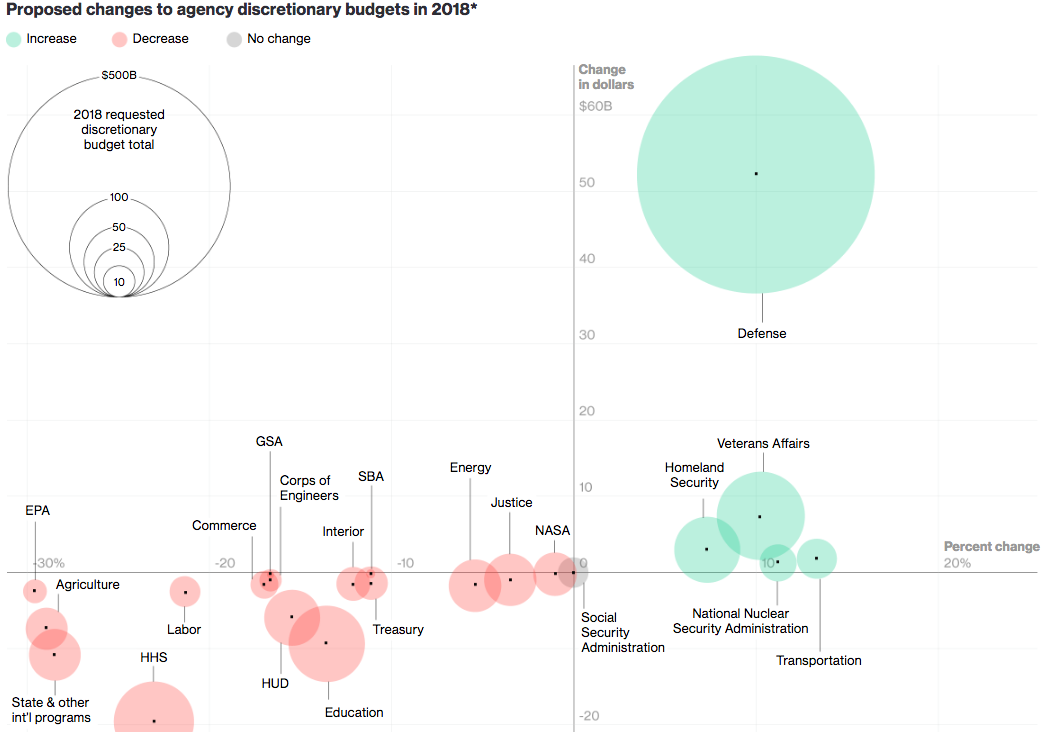
\includegraphics[scale=0.3]{budget-2018.png}
     \end{center}
\end{frame}

%@@@@@@@@@@@@@@@@@@@@@@@@@@@@@@@@@@@@@@@@@@@@@@@@@
\begin{frame}
\frametitle{Information}
\begin{itemize}
\item Suboptimal production of information;
\bigskip
\bigskip
\bigskip
\item Suboptimal consumption of information;
\bigskip
\bigskip
\bigskip
\item Decrease transaction costs (e.g. Coase Thm).
\end{itemize}

\end{frame}

%@@@@@@@@@@@@@@@@@@@@@@@@@@@@@@@@@@@@@@@@@@@@@@@@@
\begin{frame}
\frametitle{Structure of Private Rights}
\begin{itemize}
\item Allocation of risk;
\bigskip
\bigskip
\bigskip
\item Manage adjudication costs;
\bigskip
\bigskip
\bigskip
\item Generate wealth effects via compensation.
\end{itemize}

\end{frame}

%@@@@@@@@@@@@@@@@@@@@@@@@@@@@@@@@@@@@@@@@@@@@@@@@@
\begin{frame}
\frametitle{Framework of Economic Activity}
\begin{itemize}
\item More government intervention to deal with:
\begin{itemize} 
\item monopoly or anti-competitive collusion;
\item market generated shifts in balance of power between labor and capital;
\item Factors that prevent efficient consumption;
\end{itemize}
\bigskip
\bigskip
\item Less government intervention because:
\begin{itemize} 
\item Too costly;
\item Existing intervention is captured;
\item Existing intervention is OBE.
\end{itemize}
\end{itemize}
\end{frame}

%@@@@@@@@@@@@@@@@@@@@@@@@@@@@@@@@@@@@@@@@@@@@@@@@@
\begin{frame}
\frametitle{Education}

\begin{center}
\Huge Problem definition!
\end{center}

\end{frame}

%@@@@@@@@@@@@@@@@@@@@@@@@@@@@@@@@@@@@@@@@@@@@@@@@@
\begin{frame}
\frametitle{Financing and Contracting}
\begin{itemize}
\item Deal with corruption or inefficiency in government contracting;
\bigskip
\bigskip
\bigskip
\item Fix inefficiencies in capital markets;
\bigskip
\bigskip
\bigskip
\item Save too-big-to-fail economic entities/consumption smooth.
\end{itemize}

\end{frame}

%@@@@@@@@@@@@@@@@@@@@@@@@@@@@@@@@@@@@@@@@@@@@@@@@@
\begin{frame}
    \begin{center}
     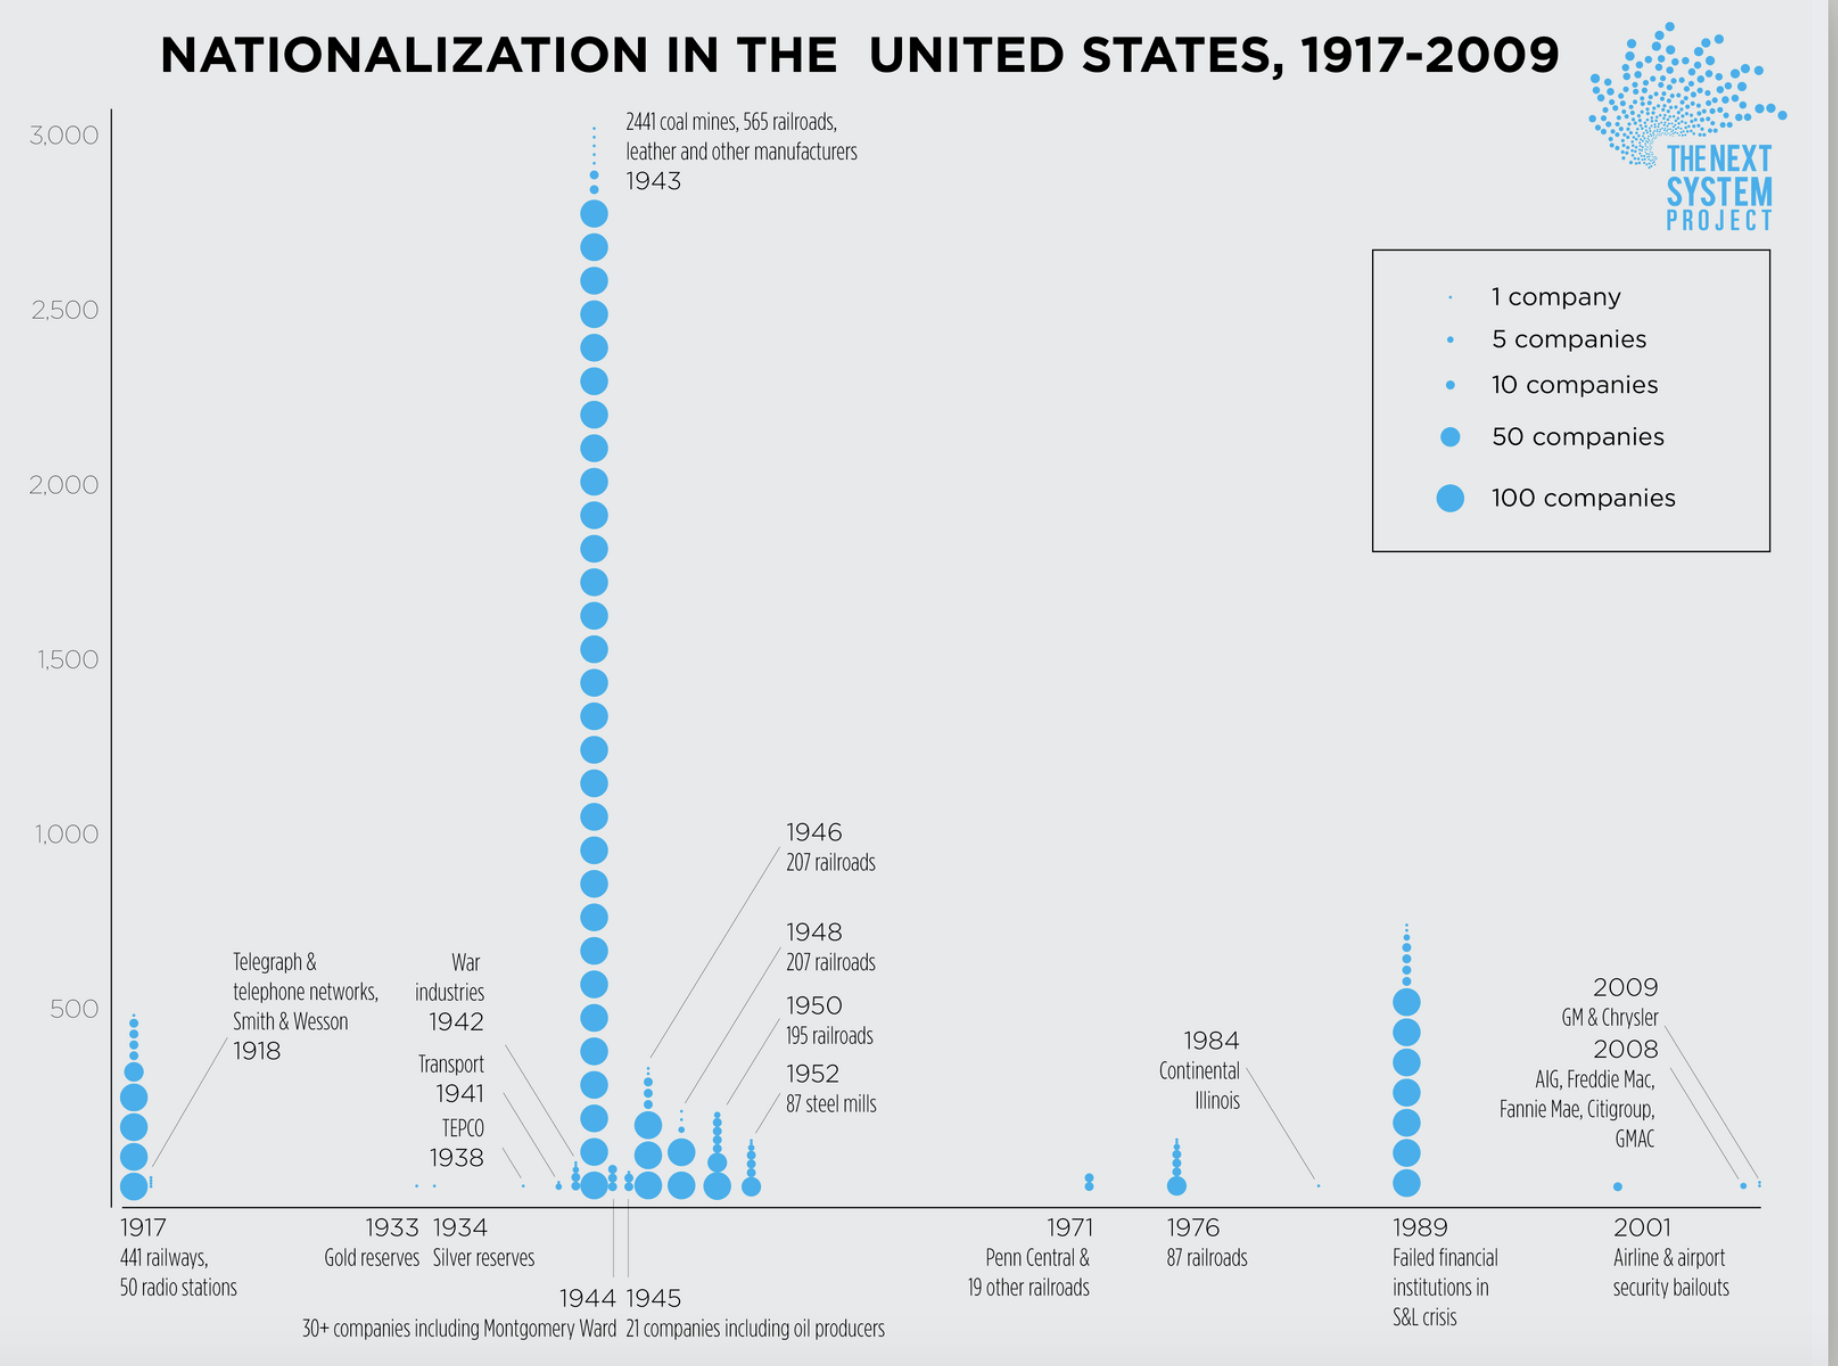
\includegraphics[scale=0.3]{nationalization.png}
     \end{center}
\end{frame}


%@@@@@@@@@@@@@@@@@@@@@@@@@@@@@@@@@@@@@@@@@@@@@@@@@
\begin{frame}
\frametitle{Bureaucratic and Political Reforms}
\begin{center}
\Huge ???
\end{center}
\end{frame}


%@@@@@@@@@@@@@@@@@@@@@@@@@@@@@@@@@@@@@@@@@@@@@@@@@
%\begin{frame}
%\frametitle{Agenda Change}
%\begin{columns}
%
%\begin{column}{0.5\textwidth}
%
%\begin{itemize}
%\item Indicators = data that can be monitored for evidence of a worsening problem;
%\bigskip
%\bigskip
%\item ``Problem streams" and ``political streams" may change rapidly due to a \textbf{focusing event}: a sudden event that can generate attention to public problems or issues, particularly issues and problems that are harmful;
%\bigskip
%\bigskip
%\item The resulting pattern of policymaking is often called \textbf{punctuated equilibrium};
%\end{itemize}
%\end{column}
%\begin{column}{0.5\textwidth}
%    \begin{center}
%     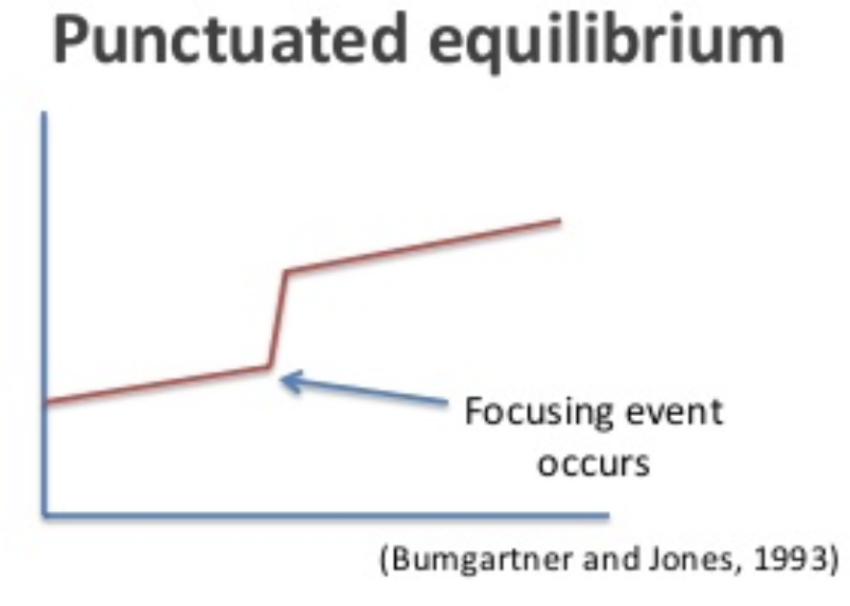
\includegraphics[scale=0.5]{punctuated_eq.png}
%     \end{center}
%\end{column}
%\end{columns}
%\end{frame}



\end{document}








